\documentclass[fleqn,useAMS,usenatbib]{mnras}
%=====================================================================
% CUSTOM: PACKAGES, MACROS & SETTINGS
%=====================================================================
% packages for figures
\usepackage{graphicx,todonotes}

% packages for symbols
\usepackage{latexsym,amssymb}

% AMS-LaTeX package for e.g. subequations
\usepackage{amsmath,morefloats}
\usepackage{natbib,graphicx,amsmath,subfigure,color}

\topmargin-1cm

\graphicspath{{figures/}}

\newcommand\notedo[1]{\todo[color=yellow, inline, size=\small]{To do:#1}}
\newcommand\notewrite[1]{\todo[color=orange, inline, size=\small]{To write: #1}}
\newcommand\noteask[1]{\todo[color=cyan, inline, size=\small]{To ask: #1}}
\newcommand\notecontrib[1]{\todo[color=green, inline, size=\small]{Contributors: #1}}
\newcommand\ess[1]{\todo[color=red, inline, size=\small]{Erin: #1}}

\newcommand{\vecg}{\mbox{\boldmath $g$}}
\newcommand{\vece}{\mbox{\boldmath $e$}}
\newcommand{\veck}{\mbox{\boldmath $k$}}
\newcommand{\vecQ}{\mbox{\boldmath $Q$}}
\newcommand{\vecF}{\mbox{\boldmath $F$}}
\newcommand{\vecD}{\mbox{\boldmath $D$}}
\newcommand{\matR}{\mbox{$\bf R$}}
\newcommand{\matC}{\mbox{$\bf C$}}
\newcommand{\bnab}{\boldsymbol{\nabla}}
\newcommand{\bnabg}{\boldsymbol{\nabla_g}}
\newcommand{\galsim}{\texttt{GALSIM}}
\newcommand{\ngmix}{\texttt{ngmix}}
\newcommand{\nnsim}{\texttt{nsim}}
\newcommand{\snr}{$S/N$}
\newcommand{\sn}{$S/N$}
\newcommand{\coadd}{{\rm coadd}}
\newcommand{\desreq}{$4\times 10^{-3}$}
\newcommand{\lsstreq}{$2\times 10^{-3}$}

\newcommand{\mcal}{\textsc{metacalibration}}
\newcommand{\Mcalshort}{\textsc{metacal}}
\newcommand{\Mcal}{\textsc{Metacalibration}}
\newcommand{\vest}{\mbox{\boldmath $e$}}
\newcommand{\est}{e}
\newcommand{\mcalR}{\mbox{\boldmath $R$}}
\newcommand{\mcalRS}{\mbox{\boldmath $R_S$}}
\newcommand{\gest}{\mbox{\boldmath $\hat \gamma$}}
\newcommand{\vecgam}{\mbox{\boldmath $\gamma$}}

\title[Metadetection]{Mitigating Shear-dependent Detection Biases with \Mcal}

\author[Sheldon et~al.]{Erin Sheldon$^1$, et al.,
  \\$^1$Brookhaven National Laboratory, Bldg. 510, Upton, NY 11973, USA 
}

\begin{document}
\date{Draft \today}
\maketitle

\begin{abstract}
    blah blah
\end{abstract}

\section{Introduction}

blah

\section{\textsc{METACALIBRATION}}

blah

\section{Shear-dependent Detection Biases}

\subsection{Bias in Simulations of Galaxy Pairs}

\begin{figure}
    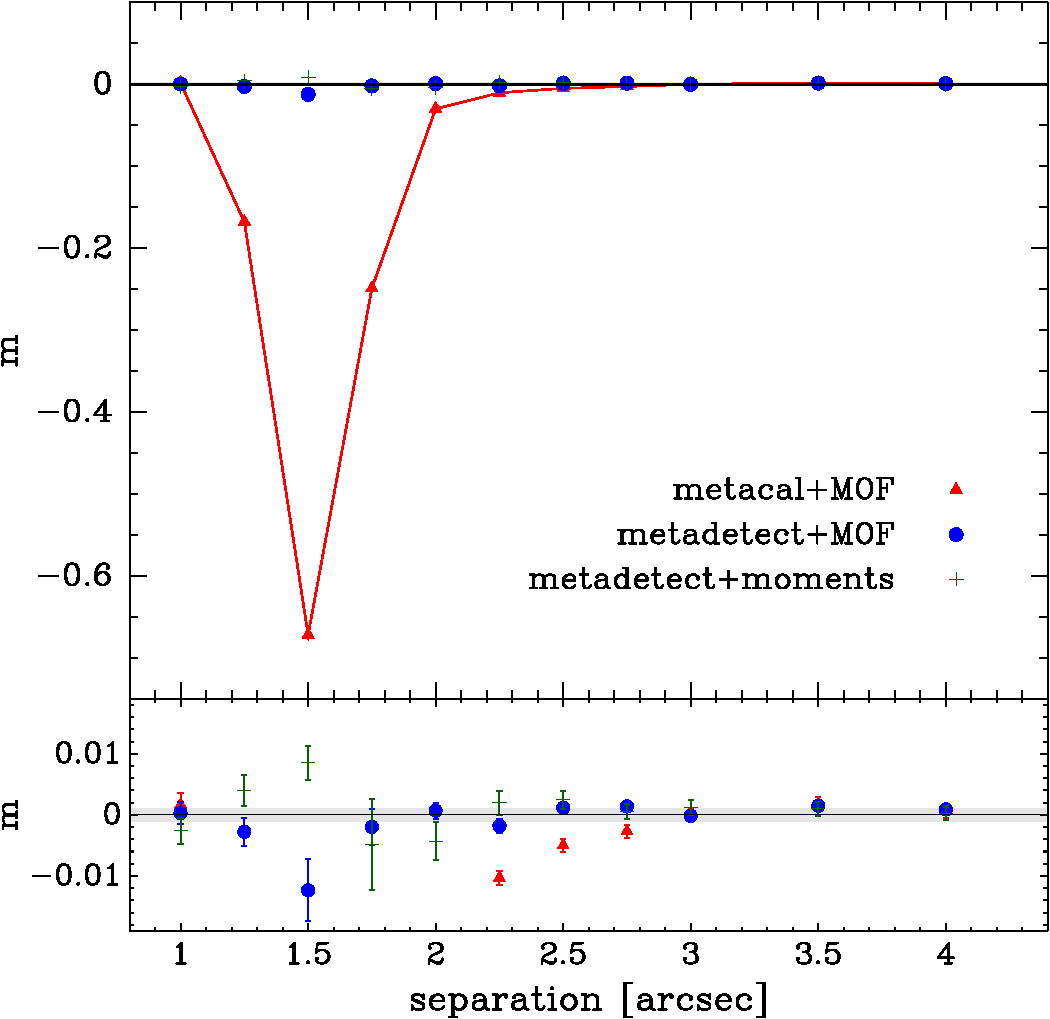
\includegraphics[width=\columnwidth]{pairs-mc-bdkpair.pdf}

\end{figure}
Erin's pair tests

\subsection{Bias in Simulations with Representative Galaxy Density and Noise}

Erin's tests with WeakLensingDeblending and Matt's tests

\section{Mitigating Shear-dependent Detection Biases with \textsc{METACALIBRATION}}
blah

\subsection{Results for Simulated Galaxy Pairs}

Erin's results with pairs

\subsection{Results for Simulations with Representative Galaxy Density and Noise}

Erin's results with WeakLensingDeblending and Matt's tests without
psf variation or masking

\subsection{Results for Simulations with Realistic Masking and PSF Variation}

Matt's stuff with the full glory

\section{Summary}
blah

\bibliographystyle{mnras}
\bibliography{references}

\end{document}
